\section{Ereignisverifizierung und -labeling für der Ereignisdaten}
Die Implementation der Ereignisverifizierung erfolgte unter der Annahmen, dass mehrere Nutzer das Tool benutzen, um Ereignisse zu verifizieren. Das Tool solle anwendbar sein, ohne das Programmierkenntnisse vom Nutzer vorausgesetzt werden müssen. Das Design legt aus diesem Grund viel Wert auf Einfachheit, Automatisierung, Fehlertoleranz und Nutzerfreundlichkeit. \par

Das Tool ist aus zwei Ebenen aufgebaut. Die Erste lässt sich als Interface für die Verifizierung betrachten und in der zweiten Ebene findet die Verifizierung statt. Die Interface-Ebene startet die Verifizierungsebene, gibt die benötigten Eingaben an diese weiter und nimmt deren Ausgabe entgegen. Die Erläuterung der Implementierung des Verifizierungstools findet in mehreren Abschnitten statt. Zunächst wird auf die Interface-Ebene eingegangen. Anschließend erfolgt die Darstellung der Verifizierungsebene. Zum Schluss wird auf einige Elemente eingegangen, welche dazu da sind, um den Grad der Automatisierung und die Fehlertoleranz erhöhen. 

\subsection{Implementation der Interface-Ebene} \label{sec:Umsetz VeriInterfaceEbene}
Die Interface-Eben lässt sich am besten anhand des Programmablaufs erklären. Dieser ist in der Abbildung \ref{fig:FlussDia IntefaceEbene} in Form eines Flussdiagramms dargestellt. Im folgenden wird auf die einzelnen Programmabschnitte im Detail eingegangen. 

\begin{figure}[p]
    \centering
    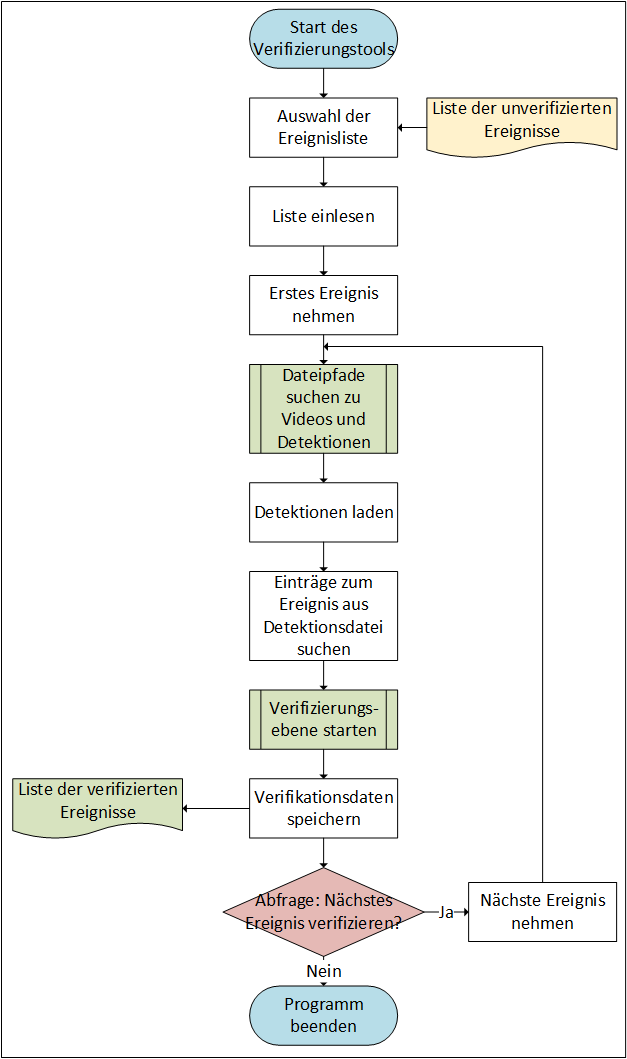
\includegraphics[height=0.9\textheight]{img/Grafiken/Flussdiagramm Interface-Ebene.png}
    \caption[Flussdiagramm des Programmablaufs der Interface-Ebene.]{Flussdiagramm des Programmablaufs der Interface-Ebene.}
    \label{fig:FlussDia IntefaceEbene}
\end{figure}

Die Ereignisse liegen als Liste in einer csv-Datei vor. Ein Ereignis ist angegeben mit Startzeitpunkt, Endzeitpunkt, Kamera ID und dem Label der Verhaltensweise. Der Aufbau der Ereignisliste ist beispielhaft in der Tabelle \ref{tab:bspUnvDataSet} dargestellt. Bei Programmstart öffnet sich ein Fenster des \textit{Datei-Explorers}, in welchem der Nutzer grafisch die Ereignisdatei suchen und auswählen kann. Das wird realisiert mit der \gls{Bibliothek} \textit{tkinter}. Eine Standardbibliothek in Python für die Erstellung von Benutzeroberflächen. Ist eine Datei mit einer Liste von Ereignissen ausgewählt, wird diese eingelesen. Das erfolgt mit der Bibliothek \textit{Pandas}. Einer weit verbreiteten Bibliothek im Bereich der Datenwissenschaften. Der Codeauszug \ref{lst:getListnLoad} zeigt das Aufrufen des \textit{Datei-Explorers}, um die Ereignisliste auszuwählen und das Laden der Liste.

\begin{pythoncode}{Auswählen der Ereignisliste über den \textit{Datei-Explorer} und Laden der Liste}{lst:getListnLoad}
import tkinter as tk
from tkinter import filedialog
import pandas as pd

#Öffnen des Datei-Explorers und 
#Dateipfad der ausgewählten csv-Datei entgegennehmen 
pfadEreignisliste = filedialog.askopenfilename(filetypes=[('csv files', '*.csv')])   

#csv-Datei der Ereignisse einlesen  
Ereignisliste = pd.read_csv(pfadEreignisliste)
\end{pythoncode}

Jede Reihe in der Liste umfasst die Daten eines Ereignisses. Iterativ wird jede Reihe aufgerufen und bearbeitet. Das Programm nimmt den Startzeitpunkt und den Endzeitpunkt des Ereignisses entgegen und stellt sicher, dass das Datumsformat das Richtige ist. Ebenfalls wird das Label und die Kamera ID entgegen genommen. Diese Angaben Initialisieren ein Objekt einer Klasse, welche als \textit{FileSearch} bezeichnet ist. Diese Klasse Implementiert die Dateisuche nach den Detektionsdateien und den Videodateien. Da diese bereits vor dieser Arbeit geschrieben wurde, wird hier nicht näher auf die Implementation der Dateisuche eingegangen. Wichtig zu wissen ist, dass \textit{FileSearch} den Start- und Endzeitpunkt eines Ereignisses, sowie die Kamera ID entgegen nimmt. Zurückgegeben wird ein \textit{FileSearch}-Objekt, mit welchem auf die gefundenen Dateipfade zugegriffen werden kann. Der Codeauzug \ref{lst:IterateSearchFiles} zeigt die Iteration durch die Liste, das Entgegennehmen eines Listeneintrags und das Übergeben der Informationen an die \textit{FileSearch}-Klasse.

\begin{pythoncode}{Iteration durch die Ereignisse und Suchen der Dateipfade.}{lst:IterateSearchFiles}
#Iterration durch die Ereignisse in der Liste
for idx, row in Ereignisliste.iterrows():  
    
    #Formatieren von  Start- und Enddatum für FileSearch
    #Ausgegebens Format dd.mm.yyyy HH:MM:ss
    startTime = format_time(row['Startdatum'])
    endTime = format_time(row['Enddatum'])

    #Entgegennehmen der Kamera ID und des Labels
    kameraID = str(row['KameraID'])
    ereignisLabel = str(row['Label'])

    #Dateien auf den Festplatten suchen und Dateipfade zurückgeben 
    files = FileSearch(startTime, endTime, kameraID)
\end{pythoncode}

Wie in \autoref{sec:Meth Labeling} beschrieben, müssen über den Detektionsdatensatz die passenden Frames zum Ereignis aus dem Video gesucht werden. Über das \textit{FileSearch}-Objekt lässt sich auf den Dateipfad zum Detektionsdatensatz zugreifen. Dieser wird mit dem gleichen Befehl geladen, wie der Ereignisdatensatz. Da es unwahrscheinlich ist, dass die Zeitangaben zu einem Ereignis exakt mit Einträgen im Detektionsdatensatz übereinstimmen, ist eine Methode notwendig, welche die Detektionseinträge sucht, die am nächsten gelegen sind zu den Zeitpunkten des Ereignisses. Ein Zeitpunkt eines Ereignisses liegt i.d.R. zwischen zwei Detektionseinträgen. Es gibt einen Eintrag der etwas früher liegt und einen der Späteren. Um sicherzustellen, das dass volle Ereignis erfasst ist, wird für den Startzeitpunkt der Frühere Eintrag gewählt und für den Endzeitpunkt der Spätere. Realisiert ist das in einer Funktion \textit{get\_closest\_timestamp}. Diese nimmt den Detetkionsdatensatz entgegen, einen Zeitpunkt und die Information, ob es sich um den Start- oder Endzeitpunkt des Ereignisses handelt. Sie sucht den passenden Detekionseintrag raus. In diesem ist die ID des Frames vermerkt, welche für die Zuordnung vom Video benötigt wird. Auch findet sich im Detektionseintrag ein Zeitstempel in Unixzeit. Vorteilhaft an der Unixzeit ist, dass sie ein eindeutiger Index für einen Detektionseintrag ist. \par

Unixzeit ist ein Zeitformat, welches Zeit als Ganzzahl darstellt. Es zählt die Sekunden (oder Millisekunden) seit dem 01.01.1970 um 00:00:00 Uhr. Durch die Darstellung als Ganzzahl ist es geeignet, um Zeitpunkte miteinander zu vergleichen.  \par

Die Unixzeit und die Frame ID werden aus der Funktion \textit{get\_closest\_timestamp} entgegen genommen. Die beschriebenen Programmabläufe sind im Codeauszug \ref{lst:loadDetsgetFrameIDs} implementiert dargestellt. Um deutlich zu machen, dass sich der Abschnitt in der Iteration durch die Ereignisse befinden, ist der Beginn der for-Schleife erneut mit in den Auszug aufgenommen. Es handelt sich nicht um einen erneuten Aufruf.

\begin{pythoncode}{Laden der Detektionen und extrahieren der passenden Zeitpunkte und Frame IDs}{lst:loadDetsgetFrameIDs}
#Iterration durch die Ereignisse in der Liste
for idx, row in Ereignisliste.iterrows():  

    #... vorheriger Code

    #Detektionen laden
    detektionen = pd.read_csv(files.detectionDataPath)

    #Einträge zum Ereignis im Detektionsdatensatz suchen
    #Zeitangaben sind im Unixformat
    unixstart, startframe = get_closest_timestamp(detektionen, startTime, 'start') 
    unixend, endframe = get_closest_timestamp(detektionen, endTime, 'end')
\end{pythoncode}

Im Codeauszug \ref{lst:startVerifygetRet} ist zu sehen, wie das Startframe, die Zeitpunkte in Unixzeit, das Ereignislabel und der Detektionsdatensatz der Verifikationsebene übergeben werden. Die Verarbeitung der Verifikationebene ist in \autoref{sec:Umsetz VeriEbene} erläutert. Zurückgegeben wird eine Liste von verifizierten Ereignissen. In der Regel besitzt die Liste nur ein einziges Element, die Informationen zu dem Ereignis, welches verifiziert werden sollte. Es gibt jedoch auch Situationen, wo es hilfreich ist, wenn mehr als ein Ereignis zurückgegeben werden kann. \par

Wie in \autoref{sec:Meth DefAufgabe} beschrieben, kann ein Kontrollgang mehrere Phasen von Aktivität umfassen. Zwischen den Phasen kehrt Normalverhalten auf. Im Ereignisdatensatz sind diese Phasen nicht vermerkt. Dort sind nur die Zeiten angegeben wann der Tierhalter den Stall betreten hat und wann er diesen wieder verlassen hat. Das ist in \autoref{sec:Meth Datensatz} erläutert. Deshalb ist implementiert, dass während eines Aufrufs der Verifikationsebene, mehrere Ereignisse verifiziert werden können. \par

Das Programm iteriert durch alle verifizierten Ereignisse und speichert diese in einer csv-Datei ab. Abgespeichert werden Start- und Endzeitpunkt, die Kamera ID und das Label. Die Zeitangaben werden von der Verifikationsebene in Unixzeit zurückgegeben. Diese werden zuvor in ein besser lesbares Zeitformat zurück konvertiert. 

\begin{pythoncode}{Übergeben der Ereignisdaten an die Verifikation.}{lst:startVerifygetRet}
#Iterration durch die Ereignisse in der Liste
for idx, row in Ereignisliste.iterrows():  

    #... vorheriger Code

    #Starten der Verifikationsebene
    verifEreignisse = verify_frames(startframe, unixstart, \ 
        unixend, files.videofilepath, detektionen, ereignisLabel)

    #Iterieren durch alle verifizierten Ereignisse 
    for ereignis in verifEreignisse:  

        #Ereignis-Informationen entgegen nehmen        
        startUnix = ereignis[0]      
        endUnix = ereignis[1]
        label = ereignis[2]

        #Unixzeit in lesbares Format konvertieren
        #dd.mm.yyyy HH:MM:SS 
        start_string, endtime_string = \ 
            get_time_string(detektionen, startUnix, endUnix)

        #Verifiziertes Ereignis abspeichern 
        save_verifEreignis(start_string, endtime_string, \ 
            kameraID, label)
\end{pythoncode}

\begin{wrapfigure}{l}{0.5\textwidth}
    \begin{center}
        \vspace*{-9mm}
        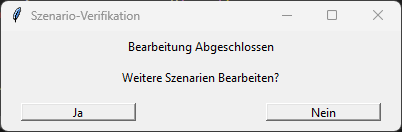
\includegraphics[width=0.5\textwidth]{img/Verifikationstool/Verifikation Abfrage Bearbeitung fortsetzen.png}
        \vspace*{-10mm}
        \caption{Fenster des Verifizierungstools für die Bestätigung der Fortsetzung der Bearbeitung.}
        \label{fig:verif BearbFortsetz}
    \end{center}
\end{wrapfigure}
Nach der Verifizierung eines Ereignisses startet die nächste Iteration durch den Ereignisdatensatz. Die Verifizierung ist zeitaufwendig. Auch die Ereignisanzahl ist hoch für eine manuelle Verifizierung. Aus diesem Grund ist es unrealistisch, dass alle Ereignisse in einer Sitzung bearbeitet werden. Um Datenverlust zu vermeiden und ein sicheres Beenden des Programms möglichst einfach zu machen, wird der Nutzer vor dem Bearbeitungsbeginn des nächsten Ereignisses gefragt, ob er die Bearbeitung fortsetzen möchte. Ist das nicht der Fall, wird das Programm sicher beendet. Anderenfalls wird das nächste Ereignis aufgerufen. Was mit dem sicheren Beenden des Programms gemeint ist, wird in \autoref{sec:Umsetz VeriZusatz} erläutert. Die Abbildung \ref{fig:verif BearbFortsetz} zeigt das Fenster mit dem der Nutzer abgefragt wird, ob die Bearbeitung fortzusetzen ist.


\subsection{Implementation der Verifizierungsebene} \label{sec:Umsetz VeriEbene}

\begin{figure}[p]
    \centering
    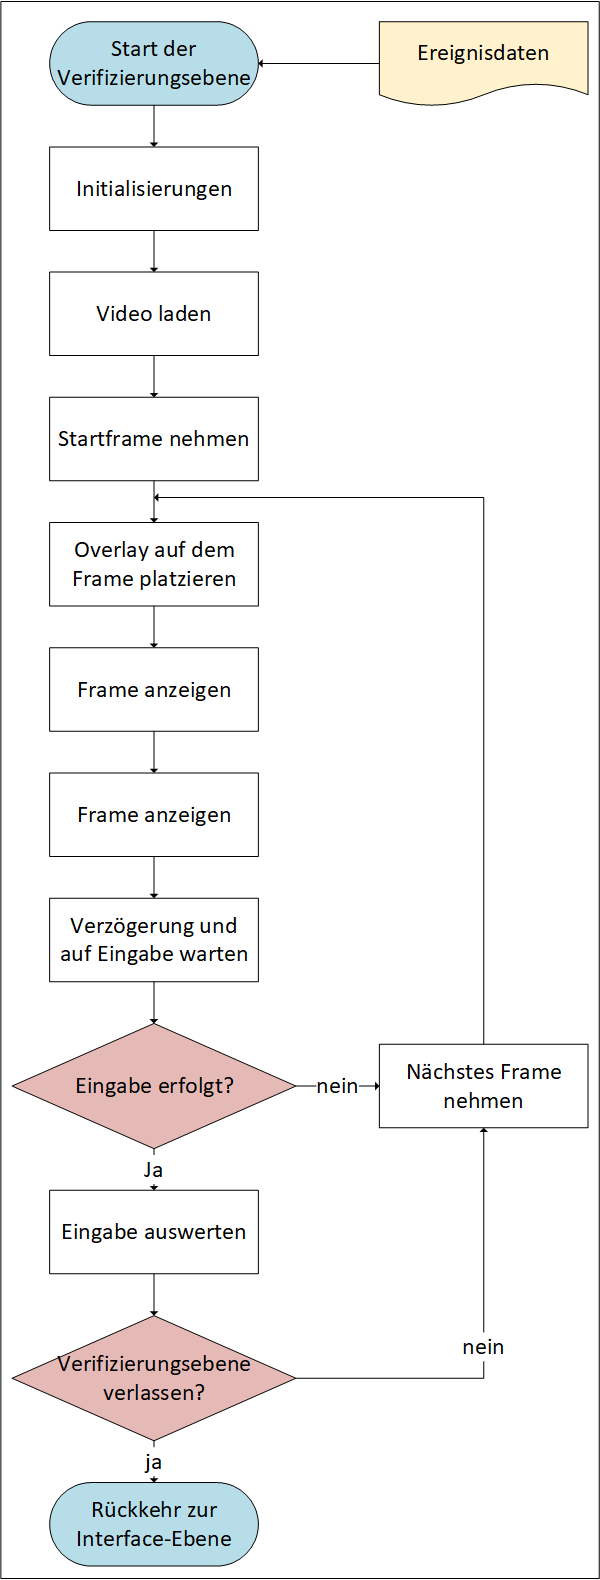
\includegraphics[height=0.9\textheight]{img/Grafiken/Flussdiagramm Verifikationsebene.png}
    \caption{Flussdiagramm des Programmablaufs der Verifizierungsebene.}
    \label{fig:FlussDia VerifyEbene}
\end{figure}

Wie in \autoref{lst:startVerifygetRet} zu sehen ist, bekommt die Verifizierungsebene die notwendigen Informationen zu einem Ereignis, um dieses zu verifizieren. Die Zeitpunktangaben und das Label dienen der Identifikation des Ereignisses. Der Detektionsdatensatz wird für die Zuordnung von Frames und Zeitpunkten benötigt, über den Dateipfad zum Video wird das Video geladen und über das Startframe kann das Video an der korrekten Position geöffnet werden. Das Flussdiagramm in der Abbildung \ref{fig:FlussDia VerifyEbene} stellt den Programmablauf der Verifizierungsebene dar. 

Wie in \autoref{sec:Meth Labeling} erläutert, soll die Verifizierung grafisch über das Video erfolgen. Um diesen Prozess nutzerfreundlich zu gestalten wird ein Overlay auf das Video gelegt. Dieses zeigt dem Nutzer wichtige Informationen über das aktuelle Ereignis, den Stand der Bearbeitung und über die Bedienung der Verifizierung. Das Overlay ist in der Abbildung \ref{fig:VerifOverlay} zu sehen. In der Abbildung \ref{fig:VerifOverlay Elem} wird auf die einzelnen Elemente eingegangen.


\begin{figure}[hp]
     \centering
     \begin{subfigure}[b]{0.9\textwidth}
         \centering
         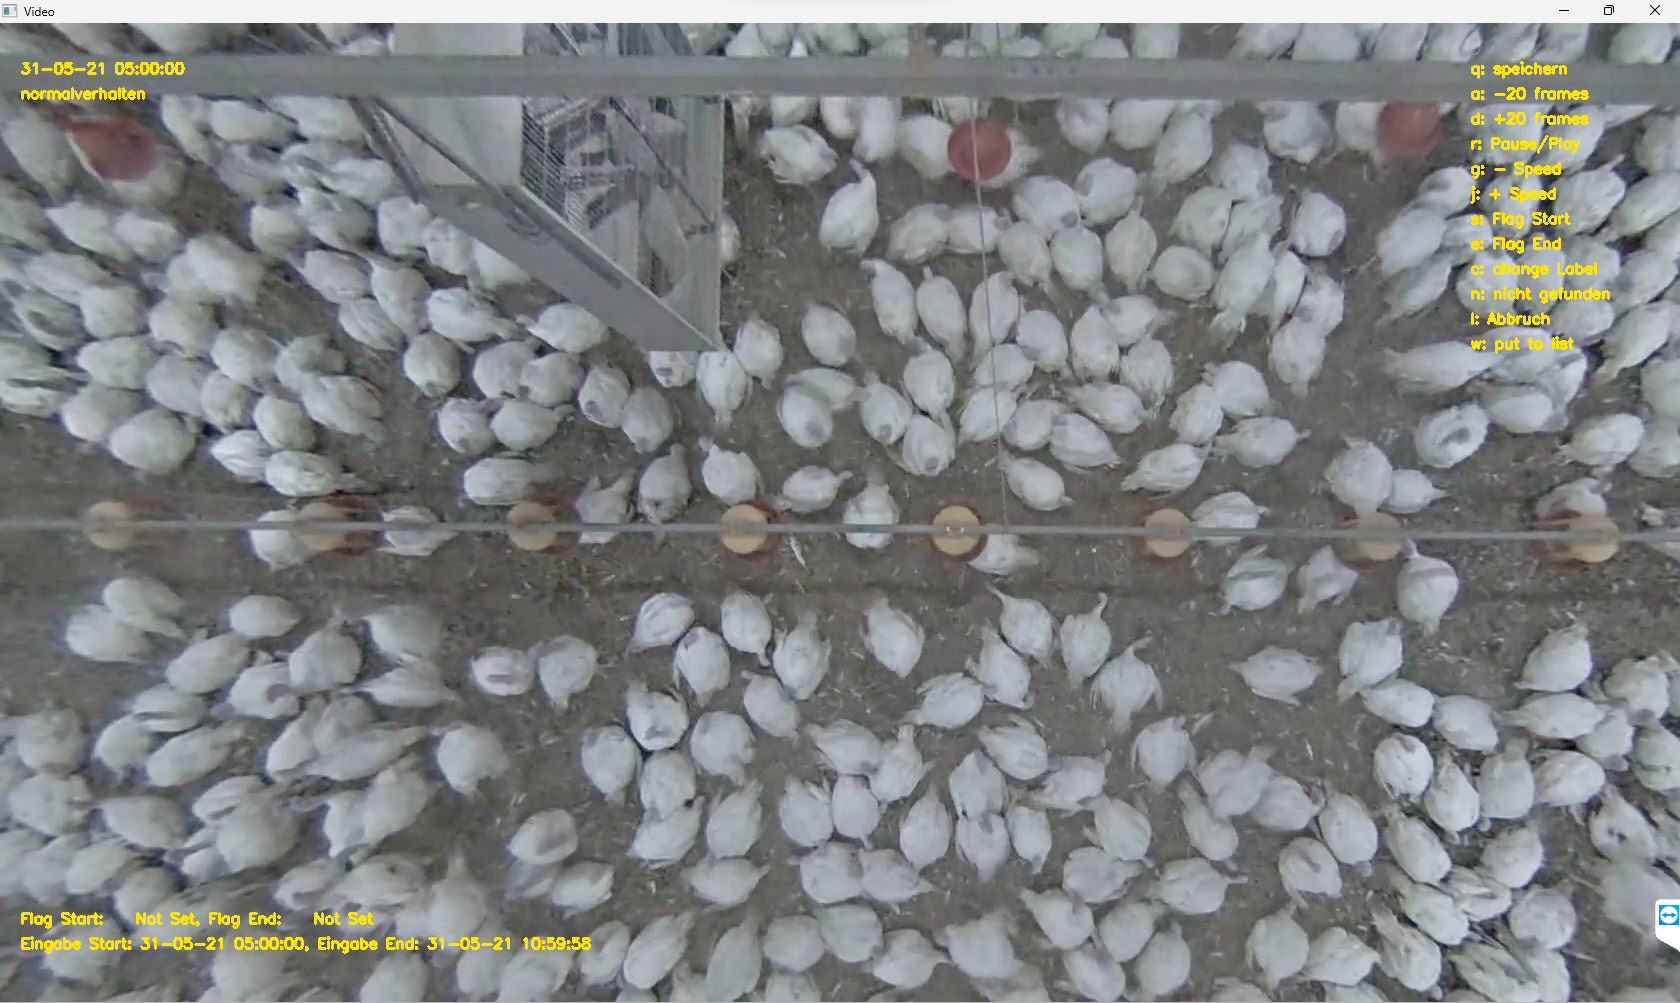
\includegraphics[width=\textwidth]{img/Verifikationstool/Verifikation Video mit Maske.png}
         \caption{Overlay des Verifizierungstools.}
         \label{fig:VerifOverlay}
     \end{subfigure}
     \hfill
     \begin{subfigure}[b]{0.9\textwidth}
         \begin{subfigure}[b]{0.59\textwidth}
             \centering
             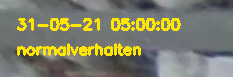
\includegraphics[width=\textwidth]{img/Verifikationstool/Verifikation Video mit Maske Uhrzeit und Label.png}
             \caption{Label und Zeitstempel des Frames}
         \end{subfigure}
         \hfill
         \begin{subfigure}[b]{0.4\textwidth}
             \centering
             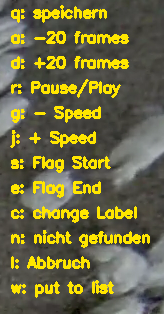
\includegraphics[width=\textwidth, height=7cm]{img/Verifikationstool/Verifikation Video mit Maske Bedienung.png}
             \caption{Bedienungshinweise}
         \end{subfigure}
     \end{subfigure}
     \begin{subfigure}[b]{0.9\textwidth}
         \centering
         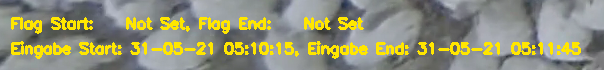
\includegraphics[width=\textwidth]{img/Verifikationstool/Verifikation Video mit Maske Ereignisinfos.png}
         \caption{Übersicht über die Ereignismarkierung. Keine gesetzten Falggen.}
     \end{subfigure}
     \hfill
     \begin{subfigure}[b]{0.9\textwidth}
         \centering
         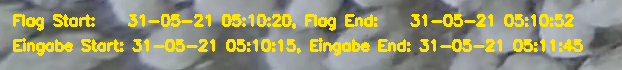
\includegraphics[width=\textwidth]{img/Verifikationstool/Verifikation Video mit Maske Ereignisinfos set.png}
         \caption{Übersicht über die Ereignismarkierung. Gesetzte Falggen.}
     \end{subfigure}
     \caption[Elemente des Overlays des Verifizierungstools.]{Elemente des Overlays des Verifizierungstools.}
     \label{fig:VerifOverlay Elem}
\end{figure}

Der Nutzer erhält über das Overlay Informationen über den betrachteten Zeitpunkt. Die Anzeige wird mit jedem Frame aktualisiert, so dass immer der korrekte Zeitpunkt zum betrachteten Frame zu sehen ist. Ebenfalls wird das Label angezeigt. Der Nutzer weis dadurch immer, welche Verhaltensweise er in der Bearbeitung zu erwarten hat. Ebenfalls sind Start- und Endzeitpunkt des Ereignis angezeigt, damit der Nutzer den erwarteten Zeitraum jederzeit als Referenz hat. Mit den Flaggen wird das Ereignis markiert. Diese muss der Nutzer mittels Tastatureingabe setzen. Die Startflagge markiert den Beginn eines verifizierten Ereignis und die Endflagge das Ende. Sind diese gesetzt bekommt der Nutzer die Zeitpunkte der Flaggen im Overlay angezeigt. \par

Im Overlay befindet sich eine Übersicht über die Bedienung der Verifizierung. Mit der Platzierung dieser Übersicht im Overlay soll die Bedienung für neue Nutzer besonders einfach gemacht werden. Aber auch für Nutzer, die mit der Anwendung bereits vertraut sind, kann diese Gedankenstütze hilfreich sein. In der Tabelle \ref{tab:VeriBedienElem} sind die Bedienelemente genauer beschrieben. Das Overlay wurde in einer Farbe mit eher geringem Kontrast zu den Puten gewählt, um nicht zu sehr vom Stallgeschehen abzulenken. 

\clearpage
\begin{longtable}{>{\bfseries} p{0.07\textwidth} p{0.15\textwidth} p{0.65\textwidth}}
% Kopfzeile auf der ersten Seite
\caption{Übersicht über die Bedienung der Verifizierung}\\
\label{tab:VeriBedienElem}\\

\textbf{Taste} & \textbf{Bezeichnung} & \textbf{Beschreibung} \\
\hline
\endfirsthead

% Kopfzeile auf den folgenden Seiten
\textbf{Taste} & \textbf{Bezeichnung} & \textbf{Beschreibung} \\
\hline
\endhead

% Fußzeile auf allen Seiten außer der letzten
\multicolumn{3}{r}{Fortsetzung auf der nächsten Seite...} \\
\endfoot

% Fußzeile auf der letzten Seite
\hline
\endlastfoot

% Subüberschriften für die Feature-Kategorien
% Hier fügen Sie Ihre Feature-Beschreibungen ein
q & Speichern & Gibt die aktuell gesetzten Flaggen und das Label zurück an die Interface-Ebene. Wurden mehrere Ereignisse verifiziert, wird die Liste dieser Ereignisse zurückgegeben.\\
\addlinespace[0.7em] % Fügt 0.7em zusätzlichen Platz ein

a & - 20 Frames & Springe 20 Frames zurück. Dient der schnellen Navigation durch das Video. Ebenfalls ist das Zurückspringen oft notwendig, um den Startzeitpunkt genau zu setzen.\\
\addlinespace[0.7em] % Fügt 0.7em zusätzlichen Platz ein

d & + 20 Frames & Springe 20 Frames vor. Dient der schnellen Navigation durch das Video. \\
\addlinespace[0.7em] % Fügt 0.7em zusätzlichen Platz ein

r & Pause/Play & Pausiere das Video, oder starte die Wiedergabe wieder. Um die Übersicht zu bewahren kann es sinnvoll sein, dass Video ganz anzuhalten. \\
\addlinespace[0.7em] % Fügt 0.7em zusätzlichen Platz ein

g & - Speed & Verlangsame die Wiedergabegeschwindigkeit. Diese Funktion dient ebenfalls dazu, den Überblick über das Geschehen zu bewahren.\\
\addlinespace[0.7em] % Fügt 0.7em zusätzlichen Platz ein

j & + Speed & Erhöhe die Wiedergabegeschwindigkeit. Diese Funktion dient der schnellen Navigation durch das Video. \\
\addlinespace[0.7em] % Fügt 0.7em zusätzlichen Platz ein

s & Flag Start & Setzen der Markierung des Startzeitpunkts eines Ereignisses. \\
\addlinespace[0.7em] % Fügt 0.7em zusätzlichen Platz ein

e & Flag End &  Setzen der Markierung des Endzeitpunkts eines Ereignisses \\
\addlinespace[0.7em] % Fügt 0.7em zusätzlichen Platz ein

c & Change Label & Ändern des Labels des Ereignis. Das ist hilfreich, um z.B. zwischen den Phasen von Kontrollgängen das Normalverhalten zu verifizieren. \\
\addlinespace[0.7em] % Fügt 0.7em zusätzlichen Platz ein

n & Nicht gefunden & Ließ sich kein Ereignis verifizieren, wird das hiermit der Interface-Ebene mitgeteilt. \\
\addlinespace[0.7em] % Fügt 0.7em zusätzlichen Platz ein

l & Abbruch & Bricht die Verifizierung ab. Die Interface-Ebene erhält dann eine leere Rückgabe. \\
\addlinespace[0.7em] % Fügt 0.7em zusätzlichen Platz ein

w & Put to List & Dient dem verifizieren mehrerer Ereignisse. Mit der Taste werden die aktuellen Start- und Endflaggen, sowie das Label einer Liste beigefügt. Die Flaggen werden zurückgesetzt und es können weitere Ereignisse verifiziert werden.\\
\addlinespace[0.7em] % Fügt 0.7em zusätzlichen Platz ein

% ... und so weiter für alle Ihre Features
\end{longtable}

Als nächstes wird Code betrachtet, mit dem die Verifizierung Implementiert ist. Wie das Flussdiagramm in \autoref{fig:FlussDia VerifyEbene} zeigt, beginnt der Programmablauf mit der Annahme der Informationen aus der Interface-Ebene und der Initalisierung. Im Codeauszug \ref{lst:VeriStartIni} ist die Umsetzung zu sehen. Es werden einige Variablen und Listen initialisiert die für den weiteren Programmablauf benötigt werden.

\begin{pythoncode}{Starten der Verifizierung und Initialisierung.}{lst:VeriStartIni}
def verify_frames(startframe, starttime, endtime, \ 
        video_path, detektionen, label):
    
    #Index vom Ereignisstart und Ende abfragen
    start_idx = detektionen[detektionen['timestamp_server'] == \ 
        starttime].index.values[0]
    end_idx = detektionen[detektionen['timestamp_server'] == \ 
        endtime].index.values[0]
    
    #Variablen zum Markieren eines Ereignisses
    start_flag_idx = None
    end_flag_idx = None
    labelCursor = 0

    #Label-Stings für das Overlay 
    #und für die Rückgabe an Interface-Ebene
    LABELS = ['unlabeled', 'normalverhalten', \ 
              'kampf', 'kontrollgang']

    #initialisieren der Liste für die verifizierten Ereignisse
    output = []

    #Initale Wiedergabegeschwindigkeit
    #Verzögert laden des nächstes Frames um 80 Millisekunden 
    PlaySpeed = 80
\end{pythoncode}

Nach der Initalisierung wird das Video über den Dateipfad geladen. Das wird mit der Bibliothek \textit{OpenCV} erreicht. \textit{OpenCV} ist eine Bibliothek für Bildverarbeitung. Sie lässt sich über den Befehl \textit{import cv2} in das Programm integrieren. Anschließend wird das Video geladen und ein Cursor wird auf die Position des Startframes des Ereignisses gesetzt. Damit kann das Video direkt an der richtigen Position geöffnet werden. Die Implementation ist im Codeauzug \ref{lst:VeriLoadVid} zu sehen.

\begin{pythoncode}{Laden des Video und Startframe heraussuchen.}{lst:VeriLoadVid}
import cv2

#Video einlesen
cap = cv2.VideoCapture(video_path)

#Cursor auf das Startframe setzen
cap.set(cv2.CAP_PROP_POS_FRAMES, startframe)
\end{pythoncode}

Das Programm kann nun auf das Video zugreifen. Es folgt die Iteration durch die Frames. Das Startframe wird über den gesetzten Cursor aus dem Video extrahiert. Der Cursor wird automatisch auf das folgende Frame gesetzt, um bei der nächsten Iteration auf dieses zuzugreifen. Die Nummer der Position des Frames wird ermittelt. Darüber wird in der Funktion \textit{putTextonFrame} auf den Detektionsdatensatz zugegriffen. Aus diesem werden die Zeitangaben entnommen für das Overlay. Generell werden in der Funktion \textit{putTextonFrame} alle Elemente des Overlays auf dem Frame platziert. Anschließend wird dem Nutzer das Frame inklusive Overlay angezeigt. Der Eindruck für den Nutzer, dass ein Video abgespielt wird, entsteht somit darüber, dass die Frames nacheinander geladen werden, das Overlay drauf platziert wird und anschließend angezeigt werden. Der Programmablauf ist schnell genug, dass der Eindruck eines fließenden Videos entsteht. Im Codeauszug \ref{lst:VeriPlaceOverlay} ist der beschriebene Ablauf implementiert zu sehen.

\begin{pythoncode}{Video abspielen und Overlay platzieren.}{lst:VeriPlaceOverlay}
#Iteration solange das Video eingelesen ist
while(cap.isOpened()):

    #Frame wird geladen und Cursor wird um eins inkrementiert
    ret, frame = cap.read()

    #Position des aktuellen Frames im Video abrufen
    current_frame = int(cap.get(cv2.CAP_PROP_POS_FRAMES))

    #Platzieren der Overlay-Elemente auf dem Video 
    ret = putTextonFrame(current_frame, start_flag_idx, \ 
            end_flag_idx)
    
    #Anzeigen des Frames mit Overlay
    cv2.imshow('Video', frame)

\end{pythoncode}

Die Wiedergabegeschwindigkeit wird über eine Zeitverzögerung erreicht. Diese ist zusammen mit der Abfrage nach der Nutzereingabe implementiert. \textit{OpenCV} stellt dafür extra eine Funktion zur Verfügung. Im Codeauzug \ref{lst:VeriStartVid} ist zusehen, dass die Variable \textit{PlaySpeed} die Zeiteinstellt, die das Programm auf eine Tastatureingabe wartet. Durch die hohe Verarbeitungsgeschwindigkeit wird hierrüber erreich, dass das Programm einen Großteil der Zeit für das Registrieren der Nutzereingaben verwenden kann. Eine schnelle Reaktion des Programms auf eine Eingabe ist die Folge, was die Nutzerfreundlichkeit erhöht.

\begin{pythoncode}{Abfrage der Nutzereingabe und Umsetzung Abspielgeschwindigkeit.}{lst:VeriStartVid}
#Iteration solange das Video eingelesen ist
while(cap.isOpened()):

     #... vorheriger Code

    #Tastatureingabe abfragen und Verzögerung der Widergabe 
    key = cv2.waitKey(PlaySpeed) & 0xFF

\end{pythoncode}

Nach dem Warten auf eine Nutzereingabe wird Evaluiert, ob ein Befehl aus der Tabelle \ref{tab:VeriBedienElem} umzusetzen ist. Ist das nicht der Fall, dann wird die nächste Iteration durchgeführt. Ist jedoch ein Befehl durchzuführen, wird je nach gedrückter Taste ein anderer Programmabschnitt ausgeführt. Der Codeauschnitt \ref{lst:VeriEvalKeys} zeigt den Großteil der in der Tabelle \ref{tab:VeriBedienElem} erwähnten Bedienungsmöglichkeiten. es wurde sich auf die wichtigsten Optionen beschränkt. \par

Das setzen der Flaggen erfolgt über den Index des Starteintrags im Detektionsdatensatz, welcher bei der Initalisierung ermittelt wurde und dem Fakt, dass jedes Frame einen Eintrag im Detektionsdatensatz enthält. Da die Detektionsdaten chronologisch geordnet sind, ist auch dort die Reihenfolge der Frames erhalten und über den Index und der Schrittdifferenz vom aktuellen Frame zum Startframe lässt sich die ID des Eintrags ermitteln. Der direkte Weg über das aktuelle Frame auf den Detektionsdatensatz zuzugreifen wäre auch eine Option, jedoch ist die einfache numerische Operation deutlich effizienter. \par

Das Label kann während der Verifizierung geändert werden. Das ist vor allem zum verifizieren von mehreren Ereignissen sinnvoll. Bei der Anwendung ist es z.B. passiert, dass laut Ereignissliste ein Normalverhalten zu verifizieren ist. Dabei wurde ein Kampf gesichtet. Um diesen mit in die Datenmenge aufzunehmen, kann einfach das Label geändert werden und das Ereignis wird in die Liste geschoben. Da das Normalverhalten zufällig, gleichverteilt auf den Zeitraum des Mastdurchlaufs verteilt wurde, wie in \autoref{sec:Meth Datensatz} beschrieben, ist das Beispielszenario nicht unwahrscheinlich. \par

Um die Verifizierungseben zu verlassen existieren drei Optionen. Bei der ersten wird die Verifikation abgebrochen. Die Interface-Ebene erhält dann ein leeres Ergebnis zurück und es werden keine Informationen gespeichert. Damit soll dem Nutzer das Beenden möglichst leicht gemacht werden. Das ist wichtig, um eine hohe Wahrscheinlichkeit für ein Ordnungsgemäßes schließen der Anwendung zu erreichen. Das Risiko für  Datenverlust wird Reduziert und die Wahrscheinlichkeit für korrekte Verifikationen steigt. Zu diesem Zweck existiert auch die Option ein Ereignis als nicht auffindbar zu markieren. Die letzte Option die Verifizierungsebene zu verlassen ist indem die verifizierten Ereignisse an die Interface-Ebene übergeben werden. 

\begin{pythoncode}{Evaluation der Nutzereingabe}{lst:VeriEvalKeys}
#Iteration solange das Video eingelesen ist
while(cap.isOpened()):

     #... vorheriger Code
     
    # 's' Zum Markieren des Startframes
    if key == ord('s'):
        start_flag_idx = start_idx + (current_frame - startframe)
    
    # 'e' Zum Markieren des Endframes
    elif key == ord('e'):
        end_flag_idx = start_idx + (current_frame - startframe)
    
    # 'c' Zum ändern des Labels
    elif key == ord('c'):
        #Cursor auf das nächste Label setzen
        label = LABELS[set_cursor(labelCursor)]

    # 'w' Zum Speichern ohne zu beenden
    # Wird für das verifizieren mehrerer Ereignisse verwendet
    elif key == ord('w'):
        output.append((start_flag_idx, end_flag_idx, label, cap))
        start_flag_idx = None
        end_flag_idx = None
    
    # 'q' Zum Beenden und speichern
    elif key == ord('q'):
        #Bei mehreren Ereignissen, alle zurückgeben.
        if len(output) > 0:
            return output
        #Ansonsten gebe nur die aktuelle Markierung zurück
        return [[start_flag_idx, end_flag_idx, label, cap]]
    
    # 'l' Zum Abbrechen der Bearbeitung, ohne Speichern
    elif key == ord('l'):
        return [[None, None, label, cap]]
    
    # 'n' Speichern, dass das Ereignis nicht gefunden wurde
    elif key == ord('n'):
        return [['not found', 'not found', label, cap]]

\end{pythoncode}



\subsection{Weitere Automatisierungen und Sicherheitsfunktionen} \label{sec:Umsetz VeriZusatz}
zusätzlich zu den in \autoref{sec:Umsetz VeriInterfaceEbene} und \autoref{sec:Umsetz VeriEbene} beschriebenen Programmabläufen sind einige Methoden implementiert, welche ausschließlich dafür da sind um die Nutzerfreunldichkeit zu erhöhen, die Fehlerwahrscheilichkeit zu reduzieren und Zeitverlust zu vermeiden. \par


\begin{wrapfigure}{l}{0.5\textwidth}
    \begin{center}
        \vspace*{-9mm}
        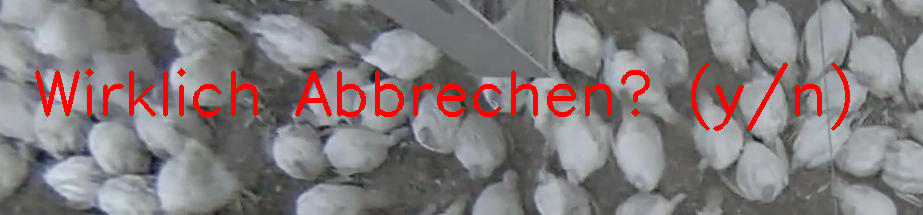
\includegraphics[width=0.5\textwidth]{img/Verifikationstool/Verifikation Video mit Maske Abbruch Abfrage.png}
        \vspace*{-10mm}
        \caption{Abfrage des Nutzers, ob die Verifizierung wirklich abgebrochen werden soll.}
        \label{fig:VerifOverlAbbruch}
    \end{center}
\end{wrapfigure}
Zunächst wird auf Zusatzmethoden in der Verifikationsebene eingegangen. Wenn verifizierte Ereignisse gespeichert werden, dann durchlaufen sie eine Kontrolle auf Korrektheit. Überprüft wird, ob beide Flaggen gesetzt sind, ob die Endflagge auf einen späteren Zeitpunkt gesetzt ist, als die Startflagge und ob ein Label ausgewählt ist. Drüber soll sichergestellt werden dass die gespeicherten verifizierten Ereignisse korrekt sind. Um ein ungewolltes Beenden zu verhindern wird der Nutzer beim  Speichern eines nicht gefundenen Ereignisses, oder bei drücken auf Abbruch, das Programm wirklich verlassen möchte. Das ist in der Abbildung \ref{fig:VerifOverlAbbruch} zu sehen. Dadurch soll verhindert werden, dass Ereignisse ungewollt nicht bearbeitet werden. Auf Grund der geringen Datenmenge ist der Verlust eines Ereignisses kritisch. \par

\begin{wrapfigure}{l}{0.5\textwidth}
    \begin{center}
        \vspace*{-9mm}
        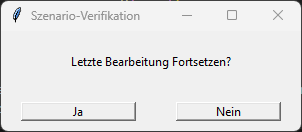
\includegraphics[width=0.5\textwidth]{img/Verifikationstool/Verifikation Abfrage Letze Bearbeitung fortsetzen.png}
        \vspace*{-10mm}
        \caption{Abfrage des Nutzers, ob er die letzte Bearbeitung fortsetzten möchte.}
        \label{fig:VeriBearbFortsetz}
    \end{center}
\end{wrapfigure}
Da die Verifizierung der Ereignisse zeitaufwendig ist, wird erwartet, dass mehrere sitzungen notwendig sind, um alle Ereignisse zu bearbeiten. Es soll sichergestellt werden, dass jedes Ereignis bearbeitet wird und auch das kein Ereignis doppelt bearbeitet wird. Aus diesem Grund wird in der Interface-Ebene, dass Abspeichern eines Zwischenstands implementiert. Es wird eine Kopie der Ereignisliste angefertigt, die der Nutzer bei Programmbeginn auswählt. Während der Verifizierung, werden die bearbeiteten Ereignisse aus dieser Kopie gelöscht. Startet der Nutzer das Programm bei einer späteren Sitzung erneut, wird er gefragt, ob die Bearbeitung dort fortgesetzt werden soll, wo zuletzt aufgehört wurde. Dazu wird auf die Kopie der Ereignisliste zugegriffen. Die Abbildung \ref{fig:VeriBearbFortsetz} zeigt das Fenster, welches Abfragt ob die letzte Bearbeitung fortgesetzt werden soll. \par

Um Datenverlust zu verhinder ist ein Backup-Mechanismus implementiert. Wird das Programm ordnungsgemäß beendet, dann wird eine Kopie der Liste der verifizierten Ereignisse erstellt. Diese Kopie wird nach dem aktuellen Datum und der Uhrzeit benannt, um den Stand zu kennzeichnen. Sollte bei einer Sitzung Fehler passieren, oder aus sonstigen Gründen die Integrität der Verifikationen aus den letzten Sitzungen fraglich sein, dann kann jeder Zeit zu einem früheren Stand zurückgekehrt werden. Das Risiko eines vollständigen Datenverlusts ist somit Reduziert. Das ist wichtig, da die manuelle Verifizierung zeitaufwendig ist und da der Zeitrahmen begrenzt ist. Ein vollständiger Datenverlust kann kritisch werden für die Umsetzung der Arbeit. 